\documentclass{article}

\usepackage{amsmath}
\usepackage{amsfonts}
\usepackage{amssymb}
\usepackage{multicol}
\usepackage{wrapfig}
\usepackage{mathenv}
\usepackage{multirow}
\usepackage{pdfpages}
\usepackage{vmargin}
\setmarginsrb{2.5cm}{2.5cm}{2.5cm}{2.9cm}{0cm}{0cm}{0cm}{0cm}

\usepackage[utf8]{inputenc}

\usepackage[french]{babel}
\selectlanguage{french}

\usepackage{color}
\usepackage{hyperref}
\hypersetup{pdfborder={0 0 0}, colorlinks=true, urlcolor=blue, linkcolor = darkred}
\usepackage{graphicx}
\graphicspath{{pdf/}} 
\usepackage{listings}
\definecolor{colKeys}{rgb}{0.75,0,0}
\definecolor{colIdentifier}{rgb}{0,0,0}
\definecolor{colComments}{rgb}{0.75,0.75,0}
\definecolor{colString}{rgb}{0,0,0.7}

\usepackage{verbatim}
\usepackage{moreverb}

\lstset{
basicstyle=\ttfamily\small, %
identifierstyle=\color{colIdentifier}, %
keywordstyle=\color{colKeys}, %
stringstyle=\color{colString}, %
commentstyle=\color{colComments}, %
showspaces=false,
}
\lstset{language=java}

% Commandes personnelles %

\definecolor{darkred}{rgb}{0.85,0,0}
\definecolor{darkblue}{rgb}{0,0,0.7}
\definecolor{darkgreen}{rgb}{0,0.6,0}
\definecolor{darko}{rgb}{0.93,0.43,0}
\definecolor{maintitle}{rgb}{0.66,0,0.22}
\definecolor{title}{rgb}{0,0.5,0.5}
\definecolor{quote}{rgb}{0.7,0.7,0.7}
\definecolor{forestgreen}{rgb}{0.14,0.54,0.13}
\definecolor{cyan4}{rgb}{0,0.54,0.54}
\definecolor{firebrick4}{rgb}{0.54,0.1,0.1}
\newcommand{\maintitlecolor}[1]{\textcolor{maintitle}{#1}}
\newcommand{\titre}[1]{\textcolor{title}{#1}}
\newcommand{\tsect}[1]{\titre{\section{#1}}}
\newcommand{\tssect}[1]{\titre{\subsection{#1}}}
\newcommand{\tsssect}[1]{\titre{\subsubsection{#1}}}
\newcommand{\vect}[1]{\overrightarrow{#1}}
\newcommand{\dred}[1]{\textcolor{darkred}{\textbf{#1}}}
\newcommand{\dgre}[1]{\textcolor{darkgreen}{\textbf{#1}}}
\newcommand{\dblu}[1]{\textcolor{darkblue}{\textbf{#1}}}
\newcommand{\dora}[1]{\textcolor{darko}{\textbf{#1}}}
\newcommand{\gre}[1]{\textcolor{darkgreen}{#1}}
\newcommand{\blu}[1]{\textcolor{darkblue}{#1}}
\newcommand{\ora}[1]{\textcolor{darko}{#1}}
\newcommand{\rouge}[1]{\textcolor{darkred}{#1}}
\newcommand{\quotecolor}[1]{\textcolor{quote}{#1}}
\newcommand{\forest}[1]{\textcolor{forestgreen}{#1}}
\newcommand{\cyan}[1]{\textcolor{cyan4}{#1}}
\newcommand{\firebrick}[1]{\textcolor{firebrick4}{#1}}
\newcommand{\ceil}[1]{\left\lceil #1 \right\rceil}
\newcommand{\cdil}[1]{\left\lfloor #1 \right\rfloor}
\newcommand{\term}[1]{\textit{\textcolor{maintitle}{#1}}}
\newcommand{\point}[2]{\item \ora{\underline{#1}} : \textit{#2}}
\newcommand{\bfp}[2]{\item \textbf{#1} : \textit{#2}}
\newcommand{\sumparam}[3]{\sideset{}{_{#1}^{#2}}\sum{#3}}
\newcommand{\sumin}[3]{\sideset{}{_{i=#1}^{#2}}\sum{#3}}
\newcommand{\sumkn}[3]{\sideset{}{_{k=#1}^{#2}}\sum{#3}}
\newcommand{\intin}[3]{\sideset{}{_{#1}^{#2}}\int{#3}}
\newcommand{\stitre}[1]{\noindent\textbf{\underline{#1}} \\}
\newcommand{\R}{\mathbb{R}}
\newcommand{\Z}{\mathbb{Z}}
\newcommand{\N}{\mathbb{N}}
\newcommand{\ualpha}{\vect{u_\alpha}}
\newcommand{\valpha}{\vect{v_\alpha}}
\newcommand{\palpha}{\vect{\Psi_\alpha}}
\newcommand{\npcomp}{\term{$\mathcal{NP}$-complet}}
\newcommand{\npcompl}{\term{$\mathcal{NP}$-complet} }
\newcommand{\cqfd}{\begin{flushright}$\square$\end{flushright}}
\newcommand{\contrad}{\begin{flushright}$\boxtimes$\end{flushright}}
\DeclareMathAlphabet{\mathpzc}{OT1}{pzc}{m}{it}
\newtheorem{de}{D\'efinition}[section]
\newtheorem{note}{Note}[section]
\newtheorem{propriete}{Propri\'et\'e}[section]
\newtheorem{exemple}{Exemple}[section]
\newtheorem{corollaire}{Corollaire}[section]
\newtheorem{interlude}{Interlude}[section]
\newtheorem{rappel}{Rappel}[section]
\newtheorem{rem}{Remarque}[section]
\newtheorem{rems}{Remarques}[section]
\newtheorem{thm}{Th\'eor\`eme}[section]
\newtheorem{lemme}{Lemme}[section]
\newtheorem{illustration}{Illustration}[section]
\newtheorem{pbm}{Problème}[section]
\newtheorem{proof}{Preuve}[section]
\renewcommand{\theproof}{\empty{}} 
\newenvironment{pblm}{\hbox{\raisebox{0.4em}{\vrule depth 1pt height 0.4pt width 5cm}}\begin{pbm}}
{\end{pbm}\hbox{\raisebox{0.4em}{\vrule depth 1pt height 0.4pt width 5cm}}}

%%%%%%%%%%%%%%%%%%%%%%%%%%%%%%%%%%%%%%%%%%%%%%%%%%%%%%%%%%%%%%%%%%%
%%%%%%%%%%%%%%%%%%%%%%%% DEBUT DU DOCUMENT %%%%%%%%%%%%%%%%%%%%%%%%
%%%%%%%%%%%%%%%%%%%%%%%%%%%%%%%%%%%%%%%%%%%%%%%%%%%%%%%%%%%%%%%%%%%

\begin{document}\begin{sffamily}


\includepdf[pages={1},offset=60 -60]{pageGarde.pdf}

\tableofcontents

\newpage

\section{Introduction}

Dans le cadre du cours ``Ergonomie des logiciels'' donné par M\textsuperscript{me} Van Daele à l'univertisé de Mons, il nous est demandé 
d'effectuer un travail en rapport avec le cours. Ce travail consiste en l'étude et l'analyse ergonomique d'un site web ou d'une application au 
choix. Le présent rapport fait état de l'analyse ergonomique du site de la \textbf{FGTB} \url{http://monaffiche.fgtb.be}, application web qu'il m'a 
été donné de développer lors de mon stage au sein de la SPRL \textbf{TagExpert}. L'analyse effectuée a pour référentiel le cours cité 
précédemment ainsi que l'écrit ``Guide ergonomique de conception des interfaces homme-ordinateur'' de Scapin et Bastien.\\

Après une brève présentation de la \textbf{FGTB} et de \textbf{TagExpert}, l'application web sera ensuite placée dans son contexte (utilité, but) 
pour finalement être analysée selon les différents critères spécifiés par le référentiel. Une conclusion jugeant la globalité des critères 
terminera ce rapport en attribuant une bonne ou une mauvaise note à l'application. 

\section{Présentation}

Cette section s'articule en 3 points, conformément au plan annoncé : présentation de la \textbf{FGTB} et de \textbf{TagExpert} et présentation de 
l'application web. Là où les deux premiers points seront très succints, le troisième point est le plus important car il s'agit de présenter le réel 
objet de ce rapport.

\subsection{La FGTB}

La \textbf{FGTB} est un syndicat qui défend tous les travailleurs. Sa spécificité est d'agir pour une société plus égalitaire, plus solidaire et sa 
force est d'allier capacité de concertation et détermination dans la défense des travailleurs. Préparer un avenir durable pour les jeunes, penser 
l’accès à l’emploi de qualité dans le souci de l’égalité entre les femmes et les hommes, autant de préoccupations mises à l’agenda par la 
\textbf{FGTB}, qui reste le moteur du syndicalisme de demain. \\

La \textbf{FGTB} défend un projet de société. Elle travaille au jour le jour à plus de justice sociale, à une meilleure répartition des richesses, 
à plus d’égalité dans le monde du travail. Elle veille aussi à pouvoir répondre aux préoccupations et inquiétudes de chacun des travailleurs, tout 
en défendant un projet de société collectif, solidaire et non corporatiste. Organisation fédérale (ailes wallonne, bruxelloise, flamande), la 
\textbf{FGTB} (Fédération Générale du Travail de Belgique) veut maintenir une sécurité sociale, une concertation sociale et un droit du travail 
forts, au niveau fédéral. Elle compte aujourd'hui 1.503.000 membres qui défendent un monde du travail qui place au centre les préoccupations 
sociales et l’intérêt du travailleur et refusent un système économique et financier du tout au profit. \\

Point de vue organisation, la \textbf{FGTB} s’articule autour de 3 interrégionales, selon la structure fédérale de l'Etat belge. En outre, elle 
comprend 17 régionales (qui regroupent les affilié(e)s par zone géographique) et 7 centrales professionnelles (qui regroupent les affilié(e)s en 
fonction du secteur d’activité).

\subsection{TagExpert}

La société \textbf{TagExpert} a été créée en 2007 par les frères \textbf{Blampain} : David et Benjamin. Elle se présente comme une société 
construisant une solution aux besoins de ses clients et concrétisant ces solutions en ligne. Il s'agit donc d'une entreprise totalement orientée 
web. Elle recueille deux parties majeures : 
\begin{itemize}
\item \blu{TagExpert.com} qui est constituée d'une équipe de web-développeurs qui réalisent et mettent en ligne des sites Internet pour les 
clients,
\item \blu{TagExpert.tv} qui est constituée d'une équipe de réalisateurs/caméramans qui réalisent des vidéos de qualité professionnelle en vue de 
faire la publicité 
d'entreprises clientes ou d'effectuer des animations flash pour dynamiser un site Internet.
\end{itemize}

De manière concrète, \textbf{TagExpert} met à disposition des services tels que la réalisation de conseil stratégique et \textit{eMarketing}, de 
sites Internet élégants et efficaces, des applications robustes sur mesure, des formations et de la production et post-production vidéos dans le 
domaine de l'Internet. La société est également une fervente supportrice de l'open-source.

\subsection{L'application web}

En vue de l'approche de la campagne 2012 des élections sociales (celles-ci ayant lieu vers le mois de juin), la \textbf{FGTB} a découvert que la 
création d'affiches électorales pour ses membres pouvait être fastidieuse et coûteuse. En conséquence, une demande est arrivée sur le bureau de 
\textbf{TagExpert} : développer une application web permettant à n'importe quel membre de la \textbf{FGTB} de construire et générer sa propre 
affiche électorale en vue d'être imprimée par la suite. L'application se devait d'être intuitive et facile d'accès car une grande partie des 
membres de la \textbf{FGTB} n'est pas coutumière de l'utilisation d'un ordinateur et encore moins d'Internet.\\

L'architecture et le design de l'application ont été convenu à l'avance via un devis dont la partie concernant l'architecture et le design est 
fournie en annexe (le design a bien été amélioré par la suite, cf les annexes suivantes). En résumé, l'application est articulée en 2 pages 
principales : 
\begin{enumerate}
\item \textbf{La page d'accueil} \\
cette page ne sert qu'à accueillir les utilisateurs, leur permettre de s'inscrire et de s'identifier.
La demande de la \textbf{FGTB} à ce sujet était très claire : pas de mot de passe, juste un identifiant unique pour chaque compte. \\

\begin{figure}[h!]
	 \begin{center}
	   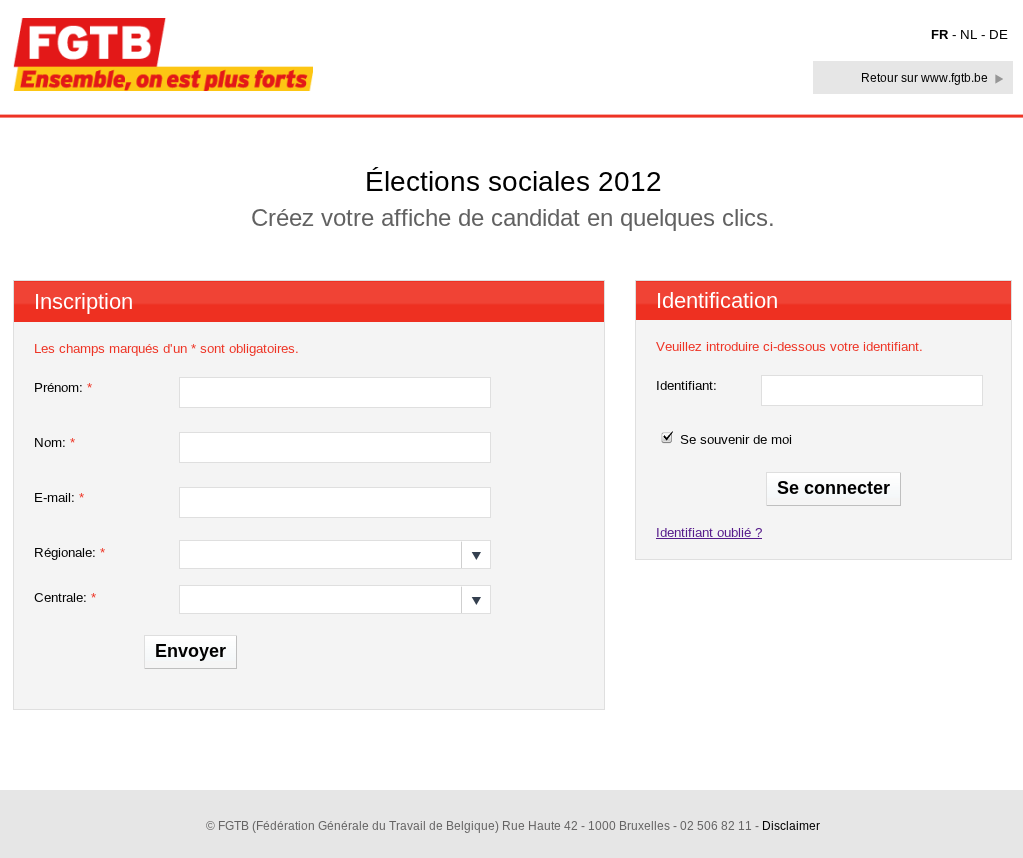
\includegraphics[width=\textwidth]{ergo_019.png} 
	   \caption{Page d'accueil}
	\end{center}
\end{figure}
\newpage
\item \textbf{La page de génération d'affiches} \\
cette page contient essentiellement 3 zones :
\begin{enumerate}
\item une table contenant les 5 dernières affiches générées permettant de les afficher, télécharger ou supprimer,
\item des onglets permettant de modifier les différentes parties de l'affiche (photo, slogan, langue, paysage/portrait),
\item un aperçu qui doit être mis à jour au fur et à mesure que des modifications sont apportées par l'utilisateur, cette zone surplombant un 
bouton imposant permettant de sauver l'affiche.
\end{enumerate}
Cette page est régit par quelques règles, comme le fait que l'utilisateur puisse uploader 5 photos et pas plus, et il en va de même pour les 
affiches générées.
\begin{figure}[h!]
	 \begin{center}
	   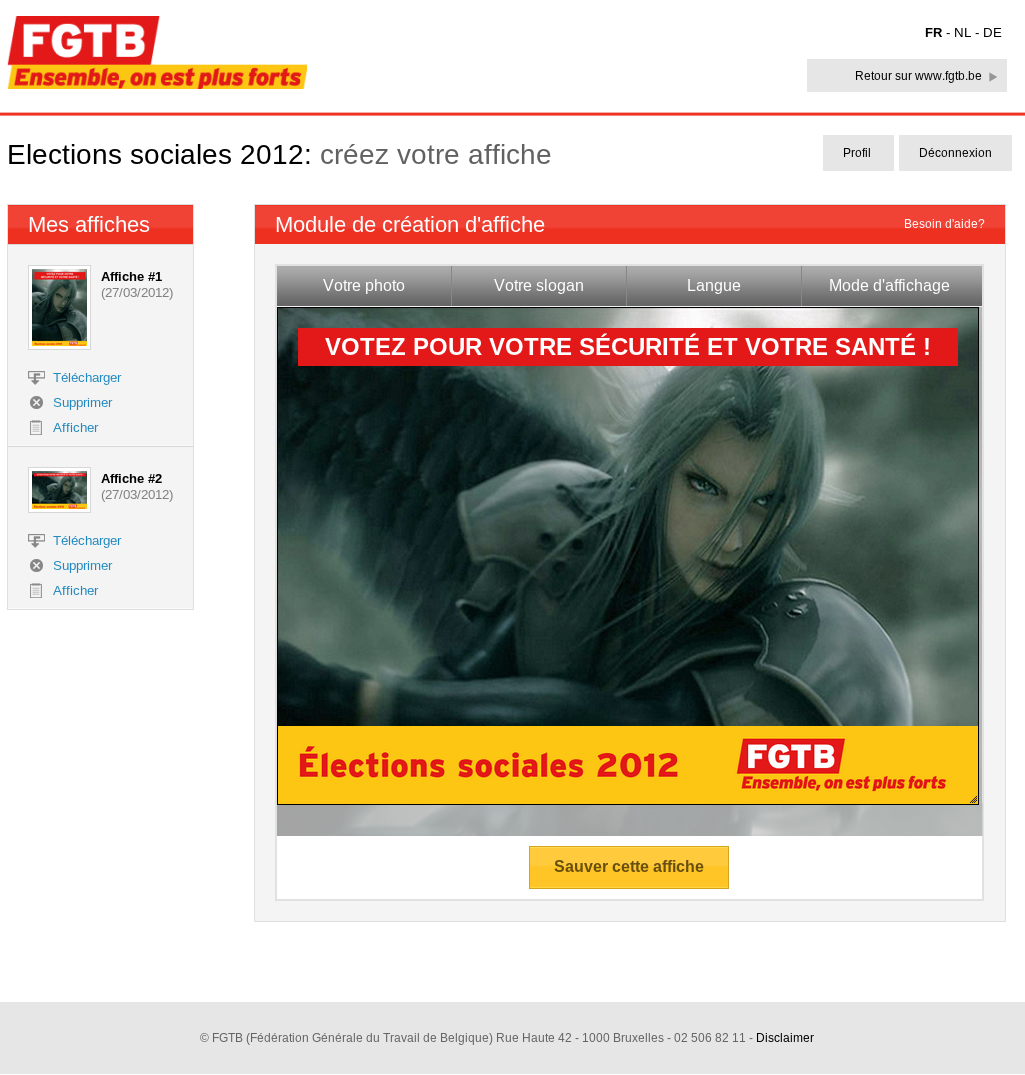
\includegraphics[width=\textwidth]{ergo_020.png} 
	   \caption{Page de génération d'affiche}
	\end{center}
\end{figure}
\end{enumerate}

\newpage

A coté de ces 2 pages principales existent 2 voire 3 pages annexes et très peu importantes :
\begin{enumerate}
\item la page d'aide qui n'est pas chargée dans une page à part mais qui apparait comme un petit pop-up lorsque l'on clique sur "Besoin d'aide ?",
\begin{figure}[h!]
	\begin{center}
		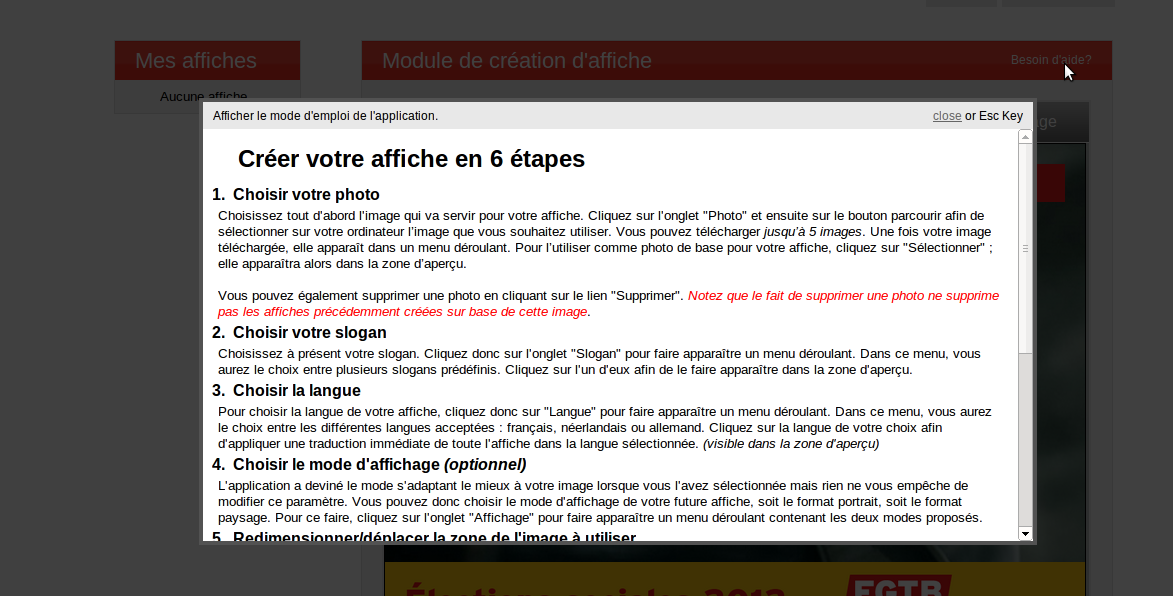
\includegraphics[width=\textwidth]{ergo_004.png} 
		\caption{Aide}
	\end{center}
\end{figure}
\item la page de récupération de l'identifiant, indispensable pour les utilisateurs ayant une petite mémoire,
\begin{figure}[h!]
	 \begin{center}
	   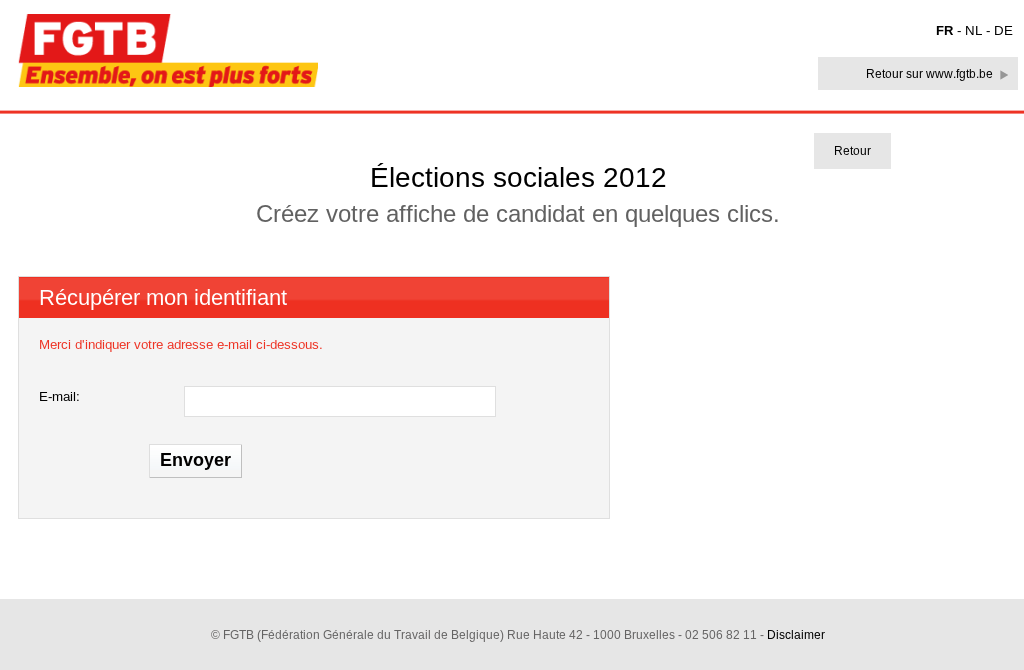
\includegraphics[width=\textwidth]{ergo_021.png} 
	   \caption{Page de récupération de l'identifiant}
	\end{center}
\end{figure}
\item la page d'édition du profil qui permet à l'utilisateur de modifier ses informations s'il change de centrale par exemple.
\begin{figure}[h!]
	 \begin{center}
	   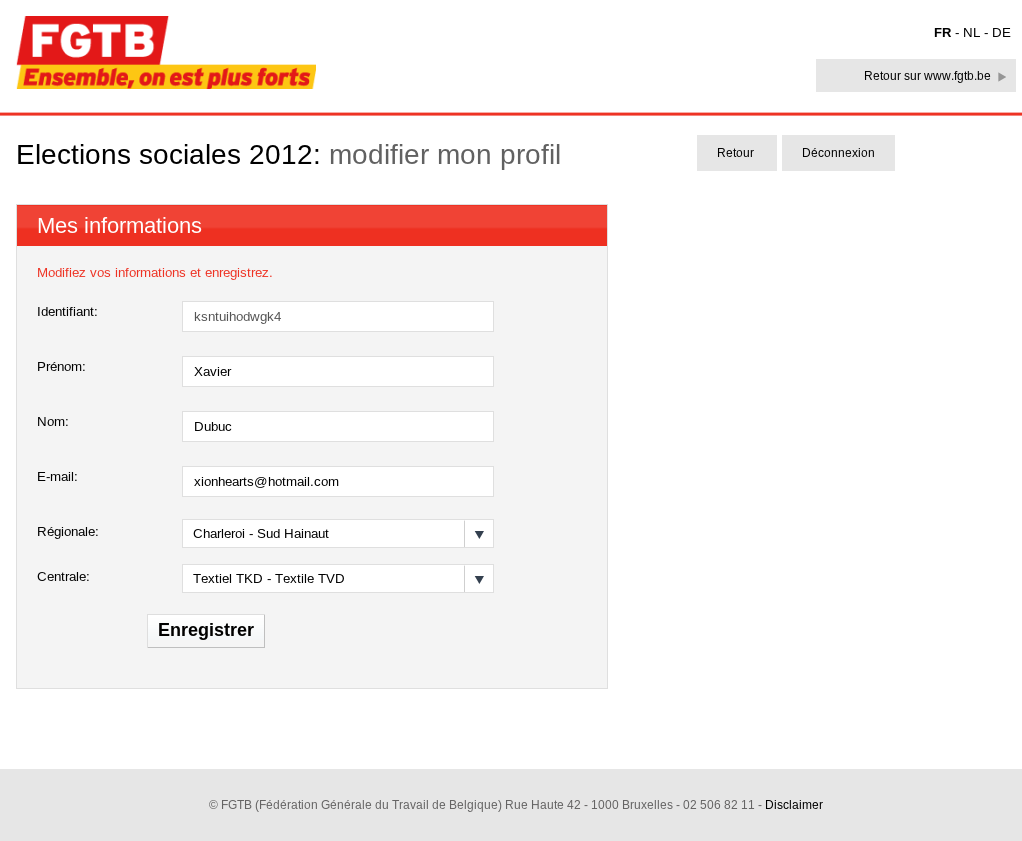
\includegraphics[width=\textwidth]{ergo_022.png} 
	   \caption{Page de modification du profil}
	\end{center}
\end{figure}
\end{enumerate}

De manière schématique, la navigation entre les différentes pages peut se représenter comme suit :

\begin{figure}[h!]
	 \begin{center}
	   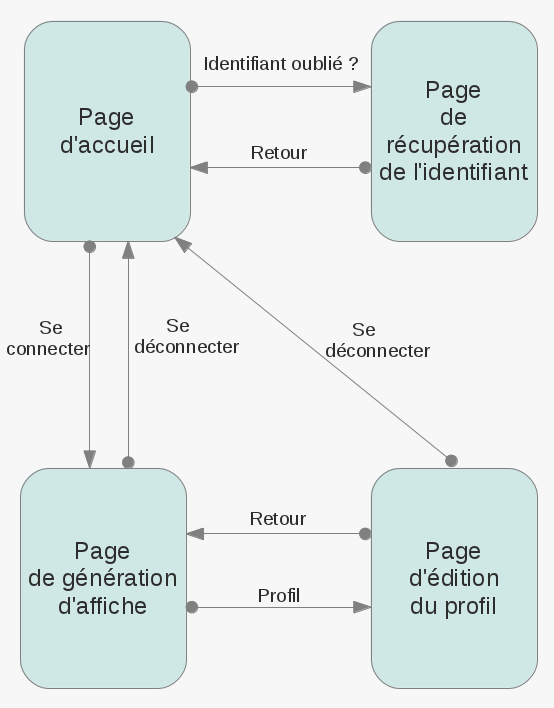
\includegraphics[width=0.25\textwidth]{ergo_023.png} 
	   \caption{Navigation entre les pages}
	\end{center}
\end{figure}

\newpage

\section{Analyse ergonomique}

Cette section regroupe les différentes observations faites sur l'application lors de l'évaluation ergonomique de celle-ci en suivant une approche analytique. Le référentiel
utilisé est celui qui nous a été conseillé lors du cours, à savoir celui de D. Scapin \& C. Bastien. Pour chaque principe (ou dimension), les critères sont passés en revue 
et s'ils ne sont pas vérifiés, une solution possible est proposée.

\subsection{Principe de guidage}


\includegraphics[scale=0.27]{good.png}

Le principe de guidage est très bien respecté au niveau de l'incitation. En effet, les 2 formulaires sont clairement bien présentés et affichent de manière évidente les deux 
choix qui se présentent à l'utilisateur : s'inscrire ou se connecter. Ces formulaires sont également bien adaptés car lorsque les choix sont limités, les champs sont des 
boites contenant ces différents choix plutôt que des champs de type "texte".

\begin{figure}[h!]
	\begin{center}
		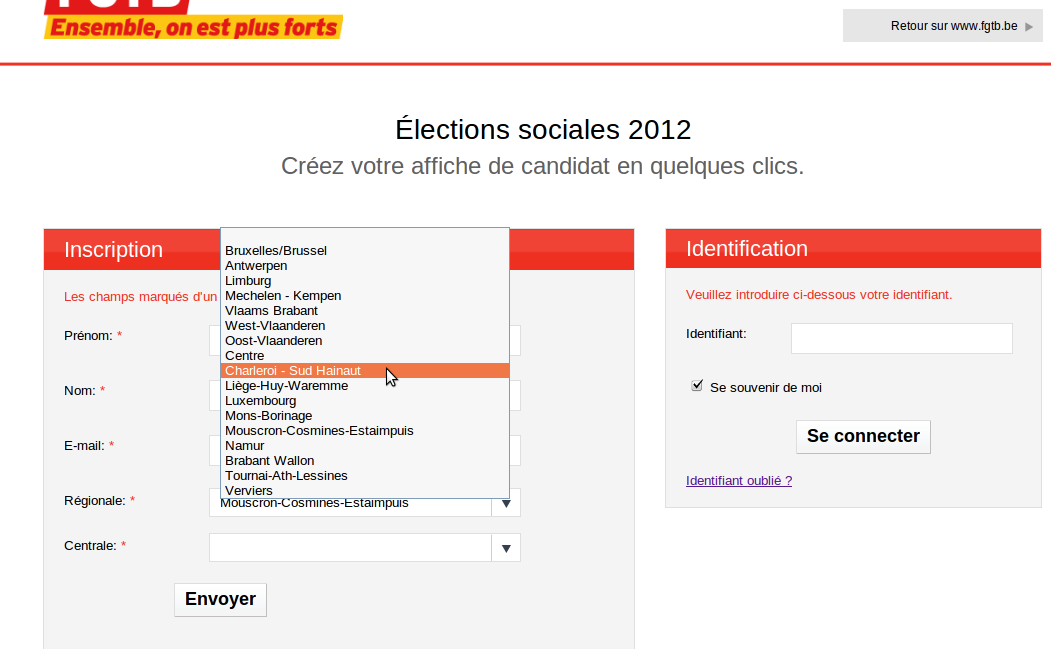
\includegraphics[scale=0.3]{ergo_001.png} 
		\caption{Page d'accueil et formulaire d'inscription}
	\end{center}
\end{figure}

Par la suite, comme on peut le voir sur la figure 8, des messages s'affichent à l'utilisateur 
lorsqu'il effectue une action irréversible comme une suppression d'image l'invitant à confirmer son choix.

\begin{figure}[h!]
	\begin{center}
		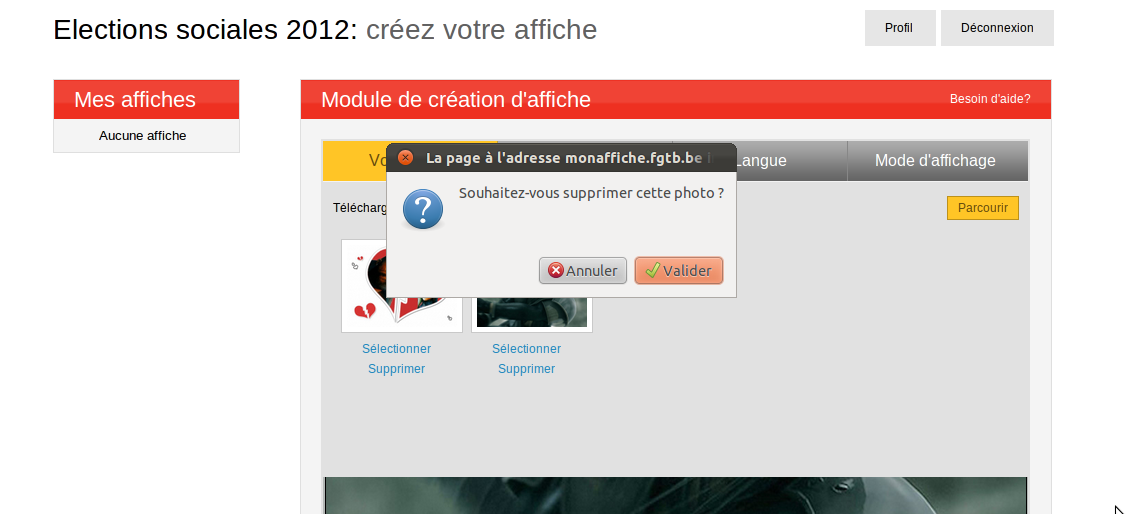
\includegraphics[scale=0.28]{ergo_003.png}
		\caption{Page de création d'affiche}
	\end{center}
\end{figure}

Il y a également une aide qui est proposée pour les personnes 
désireuses d'utiliser l'application (en cliquant sur "besoin d'aide", cf figure 9).

\begin{figure}[h!]
	\begin{center}
		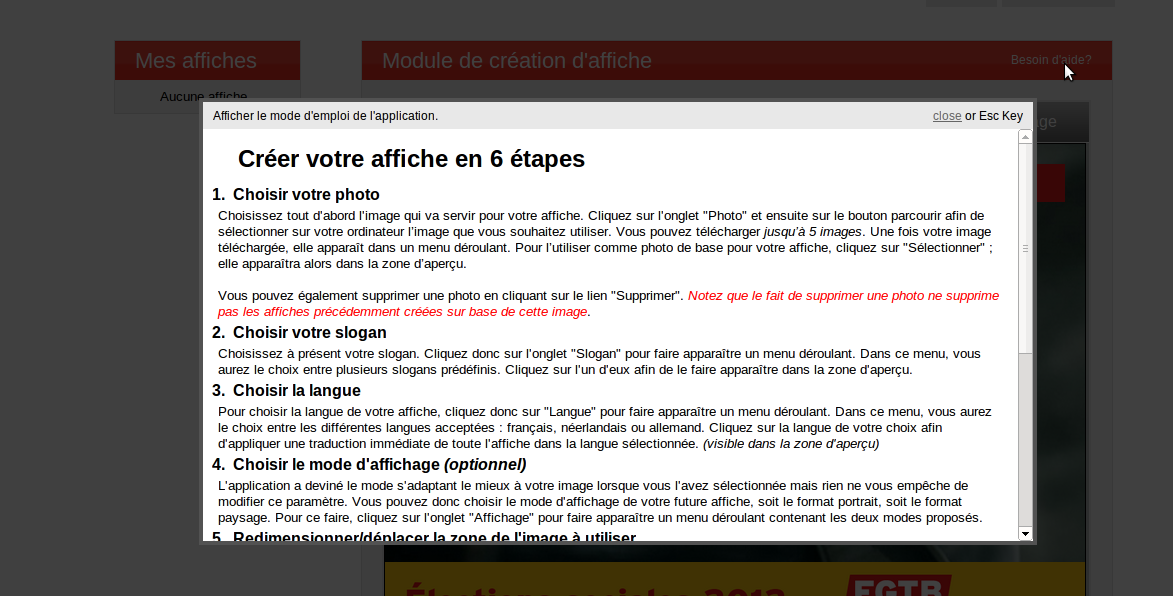
\includegraphics[scale=0.3]{ergo_004.png} 
		\caption{Aide}
	\end{center}
\end{figure}

Le groupement par localisation/format est également appliqué. En effet les onglets permettant la modification de l'affiche sont tous regroupés au même endroit et celui qui a 
été activé est d'un format différent. De plus, lorsqu'aucune image n'est chargée, le bouton "Sauver cette affiche" devient gris et ne peut plus être activé.

\begin{figure}[h!]
	\begin{center}
		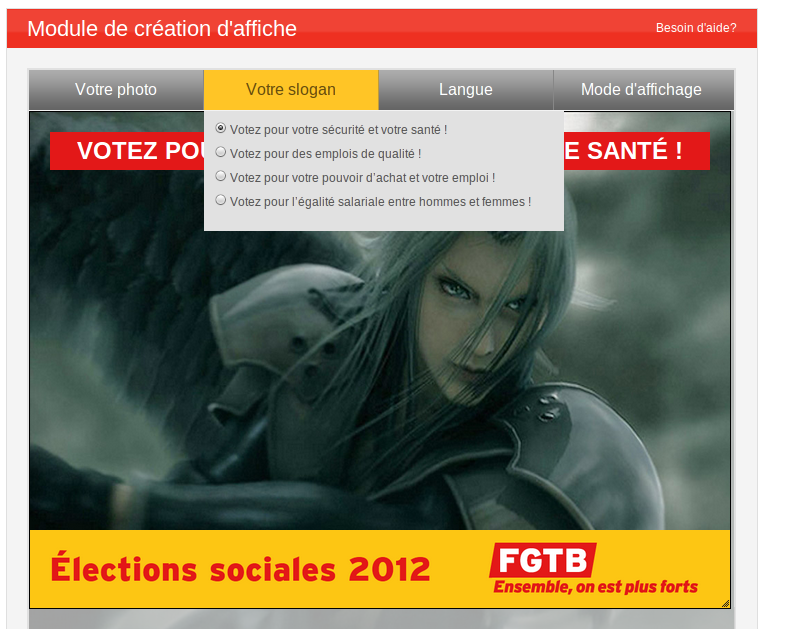
\includegraphics[scale=0.3]{ergo_006.png} 
		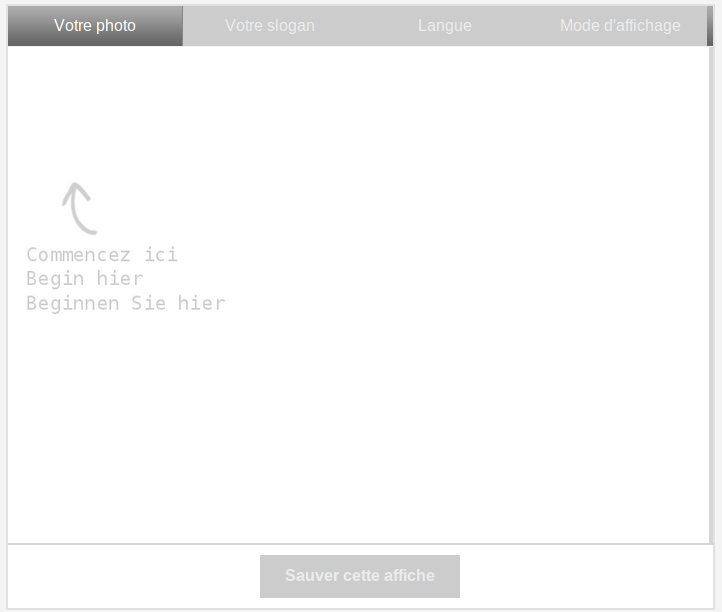
\includegraphics[scale=0.29]{ergo_007.png} 
		\caption{Groupement par localisation/format appliqué aux onglets et boutons}
	\end{center}
\end{figure}

En ce qui concerne le feedback, la zone d'aperçu est mis à jour à la seconde même où l'utilisateur modifie celui-ci via les onglets prévus à cet effet. Ceci est donc un très 
bon point car l'utilisateur peut visualiser son affiche avant même qu'elle ne soit réellement générée. La génération peut quant à elle prendre un peu de temps (jamais plus 
de 10 secondes), celle-ci dépendant de la qualité et de la taille de l'image utilisée. Un message spécifiant que la génération est en cours est alors affiché à l'écran, 
invitant l'utilisateur à patienter quelques instants. Nous serions en droit d'imaginer rajouter une phrase précisant le délai maximum d'attente ou une barre de progression 
plutôt qu'une simple animation montrant que l'application est en plein chargement. \\

\begin{figure}[h!]
	\begin{center}
		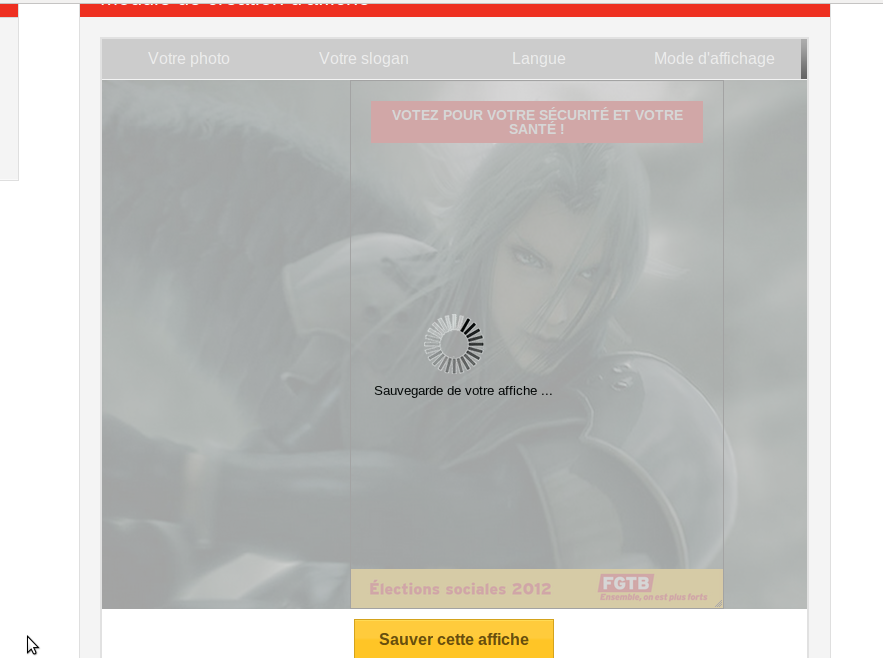
\includegraphics[scale=0.3]{ergo_005.png}
		\caption{Feedback lors de la génération d'affiche}
	\end{center}
\end{figure}

Il apparaît également de manière claire que l'entièreté du site est d'une lisibilité impeccable. Il n'y a effectivement jamais de texte trop longs 
ni trop courts, l'aide est bien structurée, les différentes phrases sont bien espacées, différentes typographies sont utilisées pour les titres, 
les sous-titres, ... \\

\subsubsection*{Résumé}

\begin{center}
\begin{tabular}{c|c|c}
\textbf{Sous-principe} & \textbf{Appréciation} & \textbf{Remarque} \\
\hline
Incitation & 
\includegraphics[scale=0.27]{good.png} & Bien respecté, partout sur le site. \\
\hline
Groupement & 
\includegraphics[scale=0.27]{good.png} & Bien respecté, partout sur le site. \\
\hline
Feedback & 
\includegraphics[scale=0.365]{mid.png} & Bien respecté sauf lors de la génération d'affiches.\\
\hline
Lisibilité & 
\includegraphics[scale=0.27]{good.png} & Bien respecté, partout sur le site. \\
\end{tabular}
\end{center}

\subsection{Principe de charge de travail}


\includegraphics[scale=0.27]{good.png}

Concernant ce principe, on peut pointer du doigt le fait que l'utilisateur peut avoir de grandes données à entrer, par exemple pour son email. Il 
pourrait être intéressant de découper l'email en 2 voire 3 parties en ne demandant pas à l'utilisateur d'entrer le "@" ni le ".". Cette pratique 
n'est cependant pas courante et pourrait déstabiliser l'utilisateur habitué à l'Internet, c'est donc plutôt un choix qu'un réel point faible à 
corriger.

\begin{figure}[h!]
	\begin{center}
		
\includegraphics[scale=0.3]{ergo_009.png}
		\caption{Champ e-mail}
	\end{center}
\end{figure}

Ceci mis à part, aucune information inutile à la tâche en cours n'est visible à l'écran (système d'onglets), les boutons et labels contiennent des 
textes simples et concis. Le système d'onglets est bien entendu prévu pour qu'un seul onglet ne soit ouvert à la fois ce qui participe grandement à 
la prise en main rapide et simple de l'application (pas de surcharge de l'écran avec des informations inutiles pour la tâche actuelle). \\

Ensuite, lors de la création de l'affiche, une affiche par défaut est générée de la façon suivante :
\begin{itemize}
\item le cadre s'adapte à la taille de l'image,
\item le premier slogan de la liste est choisi,
\item la langue "locale" (la langue utilisée par le navigateur pour afficher la page) est appliquée à l'affiche,
\item le format de l'affiche est choisi selon le format de l'image initiale.
\end{itemize}
L'utilisateur est ensuite libre de modifier chacune de ces options, de déplacer et redimensionner le cadre de l'affiche. Si l'utilisateur ne désire 
rien modifier (souvent le cadre se place exactement comme désiré, il ne reste qu'à changer le slogan), il n'a donc plus qu'à cliquer sur "Sauver 
cette affiche". Cette affiche par défaut permet donc de limiter les actions effectuées par l'utilisateur et donc les étapes par lesquelles il doit 
passer pour la génération de sa propre affiche.\\

\begin{figure}[h!]
	\begin{center}
		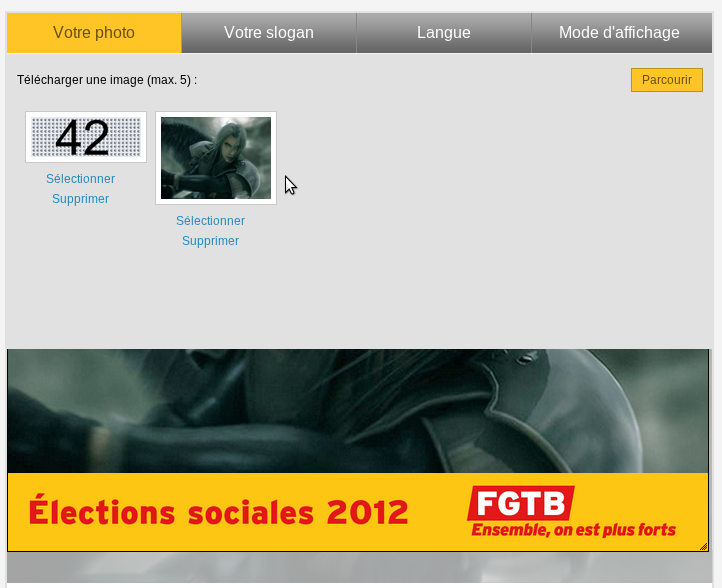
\includegraphics[scale=0.31]{ergo_017.png}
		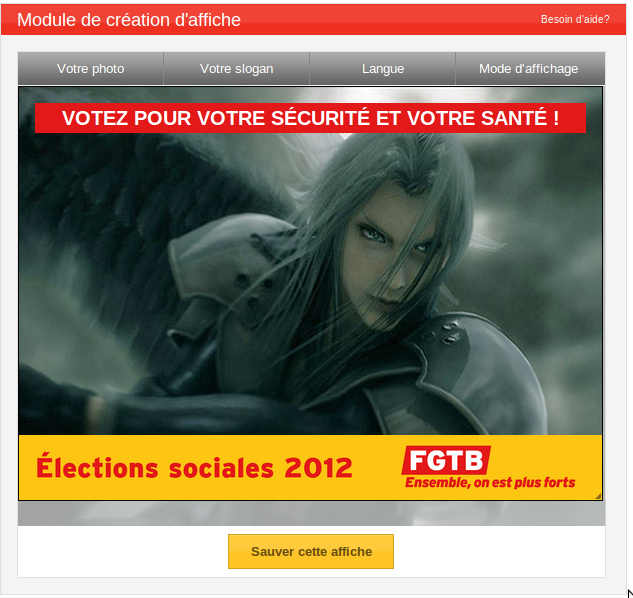
\includegraphics[scale=0.3]{ergo_008.png}
		\caption{Système d'onglets \& Affiche par défaut}
	\end{center}
\end{figure}

Au niveau de la densité informationnelle, on peut également remarquer que :
\begin{itemize}
\item les informations concernant l'aboutissement d'une tâche (création d'un compte, affiche générée, ...) sont placées en haut de la page afin 
qu'elles ne puissent être négligées,
\item les boites de sélection sont triées par ordre de fréquence,
\end{itemize}

\begin{figure}[h!]
	\begin{center}
		
\includegraphics[scale=0.3]{ergo_010.png}
		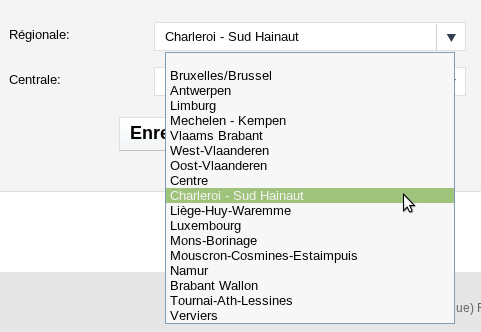
\includegraphics[scale=0.3]{ergo_018.png}
		\caption{Exemple d'information importante et ordre des boites de sélections}
	\end{center}
\end{figure}

\subsubsection*{Résumé}

\begin{center}
\begin{tabular}{c|c|c}
\textbf{Sous-principe} & \textbf{Appréciation} & \textbf{Remarque} \\
\hline
Concision & 
\includegraphics[scale=0.365]{mid.png} & Aussi bref que possible, sauf pour l'e-mail. \\
\hline
Actions minimales & 
\includegraphics[scale=0.27]{good.png} & Actions par défaut, 2-3 clics maximum pour atteindre ce qui est désiré.\\
\hline
Densité informationnelle & 
\includegraphics[scale=0.27]{good.png} & Données regroupées par fréquence et données critiques bien placées. \\
\end{tabular}
\end{center}

\subsection{Principe de contrôle explicite}


\includegraphics[scale=0.365]{mid.png} \\

Ce principe n'est pas totalement respecté. Il l'est en partie car aucune action n'est entreprise sans que l'utilisateur ne l'ait demandé. Ainsi la page affichée reste 
affichée tant que l'utilisateur ne l'a pas décidé autrement. Cependant, aucune interruption des tâches n'est possible, une fois l'action lancée il faut attendre qu'elle soit 
terminée (ou alors interagir via le browser pour empêcher l'envoi de données ou le rafraîchissement de la page). Seules les tâches de suppression d'affiche ou d'image 
recquièrent une confirmation et permettent donc leur annulation.

\subsection{Principe d'adaptabilité}


\includegraphics[scale=0.365]{bad.png}\\

Ce principe est le majeur point noir de l'application. En effet, aucune adaptabilité n'a été décelée, l'application est identique pour 
tous les utilisateurs (une seule manière de faire chaque chose) et ne permet aucune personnalisation (si ce n'est les images utilisées pour générer des affiches).

\subsection{Principe de gestion des erreurs}


\includegraphics[scale=0.27]{good.png} \\

La protection contre les erreurs est une des qualités de cette application. En effet, chaque champ est controlé avant soumission de formulaire et 
un message d'erreur apparaît afin de préciser à l'utilisateur l'erreur commise. Il y a également des infobulles s'affichant et expliquant de 
manière brève l'élément survolé par la souris de l'utilisateur. Mais aussi, comme dit précédemment, les actions irréversibles sont dotées d'un 
message demandant la confirmation avant d'effectuer cette action.

\begin{figure}[h!]
	\begin{center}
		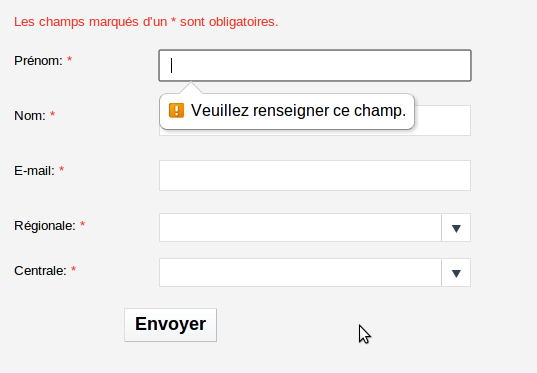
\includegraphics[scale=0.4]{ergo_011.png}
		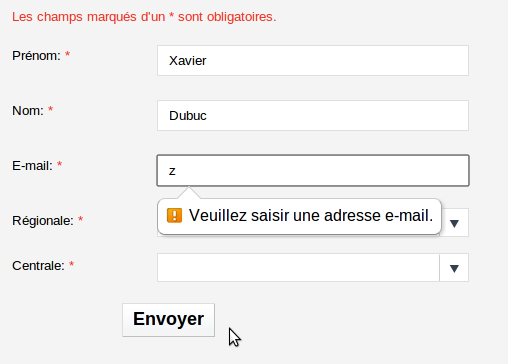
\includegraphics[scale=0.4]{ergo_012.png}
		\caption{Message indiquant les champs requis et messages d'erreurs des formulaires}
	\end{center}
\end{figure}

Il est également à remarquer qu'après chaque action nécessitant une quelconque action du serveur (création de compte, génération d'une affiche, 
...) un message soit d'erreur soit d'information apparaît et permet à l'utilisateur de savoir si sa demande a été traitée correctement et ce qu'il 
doit faire en cas d'erreur lors du traitement de celle-ci.

\begin{figure}[h!]
	\begin{center}
		
\includegraphics[scale=0.3]{ergo_010.png}
		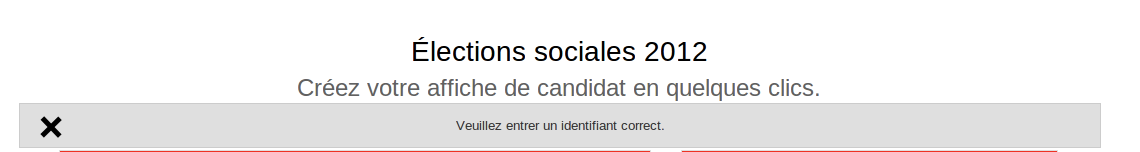
\includegraphics[scale=0.2]{ergo_013.png}
		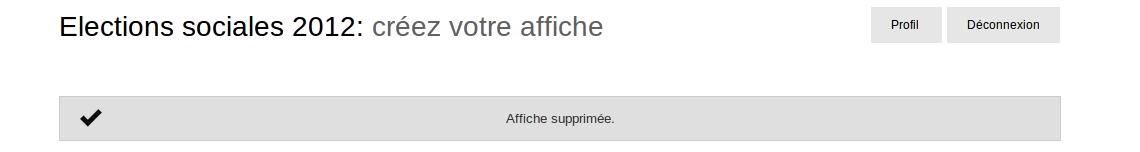
\includegraphics[scale=0.225]{ergo_014.png}		
		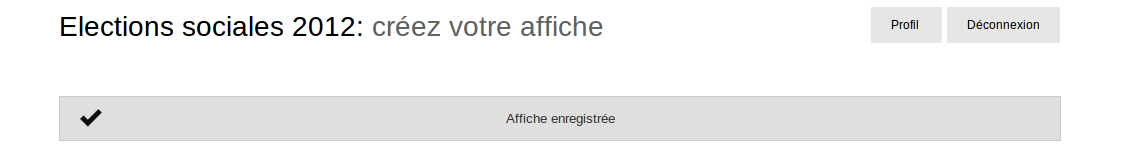
\includegraphics[scale=0.225]{ergo_015.png}
		\caption{Messages d'informations/erreurs}
	\end{center}
\end{figure}

\begin{center}
\begin{tabular}{c|c|c}
\textbf{Sous-principe} & \textbf{Appréciation} & \textbf{Remarque} \\
\hline
Protection des erreurs & 
\includegraphics[scale=0.27]{good.png} & Bulles/textes d'aide, champs contrôlés. \\
\hline
Qualité des messages d'erreur & 
\includegraphics[scale=0.27]{good.png} & Indiquent clairement à l'utilisateur que faire. \\
\hline
Correction des erreurs & 
\includegraphics[scale=0.27]{good.png} & Retour en arrière automatique après une erreur \\
\end{tabular}
\end{center}

\subsection{Principe d'homogénéité/de cohérence}


\includegraphics[scale=0.27]{good.png} \\

Comme déjà démontré au sein des précédentes sections, l'application est totalement homogène. Chaque titre de section est en blanc sur rouge, chaque 
message d'information ou d'erreur est en noir sur gris avec une croix pour les erreurs et un "v" pour les informations. Il en va de même pour les 
titres des onglets, les titres des affiches, ...Il est facilement remarquable qu'en ce qui concerne le placement de ces éléments, il est également 
constant : tout est trouvable au même endroit, peu importe la page où il est affiché.

\subsection{Principe de signifiance des codes}


\includegraphics[scale=0.365]{mid.png}

La signifiance des codes est un principe assez bien respecté dans l'ensemble. En effet, comme le montre la figure 17, on peut voir que les logos utilisés sont représentatifs 
de l'action désignée. Afin de dissiper tout doute, ils sont associés à un verbe (et nom des mots verbaux pour ne pas allonger inutilement le label) explicitant clairement 
l'action. Si ceci n'est toujours pas clair, une infobulle d'aide apparaît lorsque l'utilisateur laisse le curseur de la souris sur le lien.

\begin{figure}[h!]
	\begin{center}
		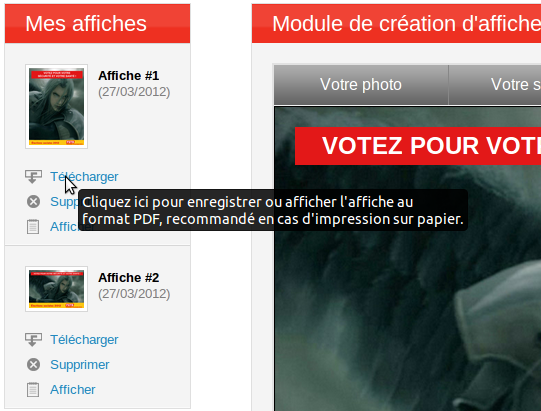
\includegraphics[scale=0.3]{ergo_016.png}
		\caption{Boutons "Télécharger", "Afficher" et "Supprimer"}
	\end{center}
\end{figure}

Le seul point faible au niveau de la signifiance des codes pourrait être le code couleur utilisé. En effet, les messages d'erreurs et 
d'informations sont affichés dans la même zone, dans la même typographie et dans la même couleur. La seule différence entre ces deux types de 
message est le logo qui apparaît au début du message (X pour les erreurs, V pour les informations). Il pourrait être judicieux d'afficher les 
messages d'erreur en rouge et/ou les messages d'information en vert ou en bleu. Ceci n'a pas été possible car la FGTB considèrait que le rouge 
était trop agressif pour les utilisateurs et ne voulait absolument pas une seule touche de bleu ou de vert sur le site Internet. Ce dernier point 
étant compréhensible car le rouge est la couleur représentative de la FGTB et le bleu serait pour le peu malvenu ... (couleur du MR (Mouvement 
Réformateur)) ! \\

\newpage

On peut cependant remarquer que les couleurs utilisées sont au nombre de 5 ce qui fait que le site ne souffre pas de l'effet "sapin de noël" et 
permet de trouver l'information désirée rapidement grâce à cela. Les couleurs associées ne font pas partie des couleurs fatiguantes pour la rétine 
une fois associées, ce qui fait un point positif de plus à soulever.

\subsection{Principe de compatibilité}


\includegraphics[scale=0.27]{good.png}

Le site s'adresse à des personnes qui ne sont pas spécialement habituées à utiliser un ordinateur et encore moins à naviguer sur Internet. Il faut donc que le vocabulaire 
utilisé soit adapté et que l'encadrement de l'utilisateur soit important. Le vocabulaire choisi est donc ciblé et bien étudié ("Télécharger", "Supprimer", "Se connecter", 
... ) et dans le cas où ces mots ne sont pas bien assimilés par l'utilisateur, une bulle d'aide apparaît sur pratiquement chaque élément de la page, permettant ainsi à 
l'utilisateur de se familiariser avec ces mots. \\

L'utilisateur a également la possibilité de se connecter et de cocher le "Se souvenir de moi" afin de limiter le nombre de fois que l'utilisateur doit fournir son 
identifiant afin de se connecter. Ceci diminue donc les informations à recoder par l'utilisateur.\\

Ces deux faits permettent de conclure que le principe de compatibilité est parfaitement respecté.

\newpage

\section{Conclusion}

En conclusion, nous pouvons porter dans un tableau les différents résultats :

\begin{center}
\begin{tabular}{c|c|p{8.5cm}}
\large{\textsc{Principe}} & \large{\textsc{Appréciation}} & \large{\textsc{Amélioration à apporter}} \\
\hline
\textbf{Guidage} & $_{
\includegraphics[scale=0.27]{good.png}}$ & Afficher une barre de progression ou une borne supérieure du 
temps d'attente lors de la génération d'une affiche.\\
\hline
\textbf{Charge de travail} & $_{
\includegraphics[scale=0.27]{good.png}}$ &  Modifier le champ e-mail en [champ]@[champ].[champ] 
même si ce n'est pas très important.\\
\hline
\textbf{Contrôle explicite} & $_{
\includegraphics[scale=0.365]{mid.png}}$ & Permettre l'annulation des tâches différentes des 
suppressions.\\
\hline
\textbf{Adaptabilité} & $_{
\includegraphics[scale=0.365]{bad.png}}$ & Prévoir une personnalisation et des raccourcis pour les 
utilisateurs aguéris.\\
\hline
\textbf{Gestion des erreurs} & $_{
\includegraphics[scale=0.27]{good.png}}$ & \\
\hline
\textbf{Homogénéité/Cohérence} & $_{
\includegraphics[scale=0.27]{good.png}}$ & \\
\hline
\textbf{Signifiance des codes} & $_{
\includegraphics[scale=0.365]{mid.png}}$ & Voir si l'instauration d'une croix rouge pour 
les messages d'erreurs et d'un V vert pour les messages d'informations est vraiment impossible.\\
\hline
\textbf{Compatibilité} & $_{\includegraphics[scale=0.27]{good.png}}$ & \\
\hline
\end{tabular}
\end{center}

$ $\\

L'application web est donc dotée d'une bonne ergonomie, elle ne possède que très peu de faiblesses. Les principaux efforts à fournir doivent 
concerner l'adaptabilité au travers d'une personnalisation possible et de raccourcis. L'application ayant été une commande de la \textbf{FGTB} à 
l'entreprise \textbf{TagExpert}, elle a été livrée avec succès aux environs du mois de février 2012 avec un contrat de maintenance en cas de 
problème majeur. Elle pourrait donc faire l'oeuvre d'un remaniage s'il est demandé par le client et jugé nécessaire par \textbf{TagExpert}.\\

On pourrait également imaginer la possibilité d'interrompre la tâche de génération d'affiche et que celle-ci affiche une barre de progression 
lorsqu'elle est executée ou tout du moins qu'elle soit annoncée comme pouvant prendre du temps en fournissant une borne supérieure ("cette action 
peut prendre jusqu'à 10 secondes"). \\

En conclusion, mis à part quelques petits détails, cette application pourrait être considérée comme modèle (au moins 
pour une majorités des critères ergonomiques) pour la création d'application semblable.

\newpage

\appendix

\section{Annexe - Partie "design" du devis}

\begin{figure}[h!]
	 \begin{center}
	   \boxed{\includegraphics[width=0.8\textwidth]{devis.png}}
	   \caption{Page 5 du devis de l'application : design de la page de génération d'affiche}
	\end{center}
\end{figure}

\section{Annexe - Revue du design (vers le milieu du projet)}

Au vue du précédent design (ce n'était qu'un prototype), on peut voir que le rendu de l'application est beaucoup plus joli et attire-l'oeil. 
L'interface semble directement plus intuitive, simple et organisée. La \textbf{FGTB} a demandé quelques modifications suite à la proposition de ce 
design, ce qui a amené au design final et actuel du site. Ces modifications concernaient surtout les couleurs. En effet, le vert a été remplacé par 
du jaune afin que les couleurs soient en accord avec la charte graphique de la \textbf{FGTB}. \\

\begin{figure}[h!]
	 \begin{center}
	   \includegraphics[width=\textwidth]{review.png} 
	   \caption{Revue du design}
	\end{center}
\end{figure}

\end{sffamily}\end{document}